\documentclass[onepage]{beamer}
\mode<presentation>{
	\setbeamercovered{transparent}
	%\beamertemplatenavigationsymbolsempty
	\setbeamertemplate{footline}[frame number]
% 	\usefonttheme{professionalfonts}
}

% https://tex.stackexchange.com/questions/34166/understanding-minipages-aligning-at-top
\usepackage{adjustbox}

% https://tex.stackexchange.com/questions/124256/how-do-i-get-numbered-entries-in-a-beamer-bibliography
\setbeamertemplate{bibliography item}{\insertbiblabel}

% https://tex.stackexchange.com/questions/49048/how-to-cite-one-bibentry-in-full-length-in-the-body-text
\usepackage{bibentry}
\bibliographystyle{plain}
\nobibliography*
%
% https://tex.stackexchange.com/questions/163827/wrong-vertical-spaces-using-bibentry-within-beamer/163842
\def\mybeamernewblock{%
  \usebeamercolor[fg]{bibliography entry author}%
  \usebeamerfont{bibliography entry author}%
  \usebeamertemplate{bibliography entry author}%
  \def\newblock{%
    \usebeamercolor[fg]{bibliography entry title}%
    \usebeamerfont{bibliography entry title}%
    \usebeamertemplate{bibliography entry title}%
    \def\newblock{%
      \usebeamercolor[fg]{bibliography entry location}%
      \usebeamerfont{bibliography entry location}%
      \usebeamertemplate{bibliography entry location}%
      \def\newblock{%
        \usebeamercolor[fg]{bibliography entry note}%
        \usebeamerfont{bibliography entry note}%
        \usebeamertemplate{bibliography entry note}}}}%
  \leavevmode
}
\newenvironment{references}{\begin{itemize}\let\newblock\mybeamernewblock}{\end{itemize}}


\setbeamersize{text margin left=10pt, text margin right=10pt}
\setbeamertemplate{itemize items}[circle]

\beamertemplatenavigationsymbolsempty

% http://tex.stackexchange.com/questions/8680/how-can-i-insert-a-newline-in-a-framebox
%\usepackage{minibox}
%\usepackage{framed}
%\usepackage[usestackEOL]{stackengine}

% % http://tex.stackexchange.com/questions/167000/annotating-tables-with-tikz-adding-arrows
% \usepackage{color, colortbl}
\usepackage{tikz}
\tikzstyle{every picture}+=[remember picture]
%\usetikzlibrary{tikzmark, positioning, fit, shapes.misc}

%% http://tex.stackexchange.com/questions/91124/itemize-removing-natural-indent
%\usepackage{enumitem}

%% http://tex.stackexchange.com/questions/41408/a-five-level-deep-list
%\usepackage{enumitem}
%\setlistdepth{9}

% https://tex.stackexchange.com/questions/20792/how-to-superimpose-latex-on-a-picture
\usepackage{overpic}

% % http://tex.stackexchange.com/questions/32661/how-to-locate-figures-with-x-y-specified-location-in-a-presentation
% \usepackage[absolute,overlay]{textpos} % absolute positioning of stuff
% \setlength{\TPHorizModule}{1mm}
% \setlength{\TPVertModule}{1mm}

\usepackage{graphicx}
\graphicspath{{../img/}}
\AtBeginDocument{\DeclareGraphicsExtensions{.eps, .png, .gif, .pdf, .jpg}}

\usepackage[makeroom]{cancel}

\usepackage[english]{babel}
\usepackage[T1]{fontenc}
\usepackage{times}

% \usepackage{amssymb}
% \usepackage{nicefrac}
% \usepackage{bbm}
% \usepackage{esint}
% \usepackage{sidecap}

\usepackage{hyperref}
% \hypersetup{pdfpagemode=FullScreen}

\newcommand{\HIDE}[1]{}

\newcommand{\skipline}{{\ }\\}

\newcommand{\EMAIL}{{\color{blue}randreev{\tiny\color{white}.\hspace{-1.5pt}}@{\tiny\color{white}.\hspace{-1.5pt}}stat.sinica.edu.tw}}

\author{\small RA}
\subject{Talks}

\newcommand{\CITE}[1]{{\footnotesize[#1]}}

% \input{definitions}

\providecommand{\DIV}{\mathop{\text{div}}}
\providecommand{\GRAD}{\mathop{\text{grad}}}

\providecommand{\IE}{\mathbb{E}}
\providecommand{\IP}{\mathbb{P}}
\providecommand{\IR}{\mathbb{R}}
\providecommand{\IZ}{\mathbb{Z}}

\providecommand{\duality}[2]{\langle #1 \rangle_{#2}}
\providecommand{\norm}[2]{\| #1 \|_{#2}}
\providecommand{\seminorm}[2]{| #1 |_{#2}}
\providecommand{\VERT}{\ensuremath{| \! | \! |}}
\newcommand{\tnorm}[2]{\VERT{#1}\VERT_{{#2}}}

\newcommand{\cA}{\mathcal{A}}
\newcommand{\cB}{\mathcal{B}}
\newcommand{\cL}{\mathcal{L}}
\newcommand{\cN}{\mathcal{N}}
\newcommand{\cT}{\mathcal{T}}
\newcommand{\cX}{\mathcal{X}}
\newcommand{\cY}{\mathcal{Y}}

\providecommand{\Abf}{\mathbf{A}}
\providecommand{\Bbf}{\mathbf{B}}
\providecommand{\Dbf}{\mathbf{D}}
\providecommand{\Ibf}{\mathbf{I}}
\providecommand{\Jbf}{\mathbf{J}}
\providecommand{\Fbf}{\mathbf{F}}
\providecommand{\Hbf}{\mathbf{H}}
\providecommand{\Mbf}{\mathbf{M}}
\providecommand{\Tbf}{\mathbf{T}}
\providecommand{\Pbf}{\mathbf{P}}
\providecommand{\Vbf}{\mathbf{V}}
\providecommand{\pbf}{\mathbf{p}}
\providecommand{\ubf}{\mathbf{u}}
\providecommand{\vbf}{\mathbf{v}}
\providecommand{\wbf}{\mathbf{w}}
\providecommand{\ybf}{\mathbf{y}}
\providecommand{\zbf}{\mathbf{z}}

\renewcommand{\vec}[1]{\mathbf{#1}}

\providecommand{\T}{\mathsf{T}}

\renewcommand{\hat}[1]{\widehat{#1}}
\renewcommand{\tilde}[1]{\widetilde{#1}}

\newcommand{\rd}{\,\mathrm{d}}

\newcommand{\TEXT}[1]{\quad\text{#1}\quad}

% http://tex.stackexchange.com/questions/211518/beamer-vfill-and-itemize
\def\Bottom#1{\vskip 0pt plus 1filll #1}
\def\BottomRight#1{\Bottom{\hfill #1}}

% MATLAB CODE LISTING
\usepackage{color}
\definecolor{DarkBlue}{rgb}{0,0,0.4}
% \definecolor{DarkRed}{rgb}{0.3,0,0}
\definecolor{DarkGreen}{rgb}{0,0.3,0}
\usepackage{listings}
\lstset{%
	language=Python,
	basicstyle=\bf\ttfamily\scriptsize,
	keywordstyle=\color{DarkBlue},
% 	numbers=left, numberstyle=\footnotesize, numbersep=4pt,
	commentstyle={\color{DarkGreen}},
% 	backgroundcolor=\color{white},
	showspaces=false, showstringspaces=false, showtabs=false,
	frame=none,
	tabsize=4,
	breaklines=true, breakatwhitespace=false,
	emphstyle={[1]\color{blue}},
	emphstyle={[2]\color{DarkGreen}},
	emph={[3]Activation,Dropout,BatchNormalization,Dense},
	emphstyle={[3]\color{red}},
	emph={[4]num_classes},
	emphstyle={[4]\color{blue}},
	xleftmargin=8pt,
	numbers=none
}


%%%%%%%%%%%%%%%%%%%%%%%%%%%%%%%%%%%%%%%%%%%%%%%%%%%%%%%%%%%%%%%%%%%%%%%%%%%%%%%%
%%
%%%%%%%%%%%%%%%%%%%%%%%%%%%%%%%%%%%%%%%%%%%%%%%%%%%%%%%%%%%%%%%%%%%%%%%%%%%%%%%%

\usepackage{ifthen}

\newcommand{\REDBOX}[1]{
	\setlength{\fboxrule}{1pt}
	\fcolorbox{red}{SeeMeBarely}{$\displaystyle
		#1
	$}
}

\definecolor{SeeMeBarely}{RGB}{230,230,230}
\definecolor{Purple}{RGB}{128,0,128}
\definecolor{DeepPurple}{RGB}{32,0,96}
\newcommand{\ra}[1]{{\color{blue}{#1}}}
\newcommand{\cred}[1]{{\color{red}{#1}}}
\newcommand{\cblu}[1]{{\color{blue}{#1}}}
\newcommand{\cpur}[1]{{\color{Purple}{#1}}}

\DeclareMathOperator*{\argmin}{arg\,min}

\newcommand{\ItemComment}[1]{\hfill{\scriptsize(#1)\normalsize}}


% http://www.webnots.com/vibgyor-rainbow-color-codes/
\definecolor{a}{RGB}{148, 0, 211}
\definecolor{b}{RGB}{75, 0, 130}
\definecolor{c}{RGB}{0, 0, 255}
\definecolor{d}{RGB}{0, 160, 0}
\definecolor{e}{RGB}{200, 200, 0}
\definecolor{f}{RGB}{255, 127, 0}
\definecolor{g}{RGB}{255, 0, 0}
%
\definecolor{z}{RGB}{0, 0, 0}
\definecolor{w}{RGB}{255, 255, 255}

% http://tex.stackexchange.com/questions/17611/how-does-one-type-chinese-in-latex
\usepackage{CJKutf8}
\AtBeginDvi{\input{zhwinfonts}}
%
\newcommand{\REN}{\begin{CJK*}{UTF8}{gbsn}人\end{CJK*}}
\newcommand{\ren}[1]{{\color{#1}\REN}}



%%%%%%%%%%%%%%%%%%%%%%%%%%%%%%%%%%%%%%%%%%%%%%%%%%%%%%%%%%%%%%%%%%%%%%%%%%%%%%%%
\begin{document}
%%%%%%%%%%%%%%%%%%%%%%%%%%%%%%%%%%%%%%%%%%%%%%%%%%%%%%%%%%%%%%%%%%%%%%%%%%%%%%%%
%%%%%%%%%%%%%%%%%%%%%%%%%%%%%%%%%%%%%%%%%%%%%%%%%%%%%%%%%%%%%%%%%%%%%%%%%%%%%%%%

%%%%%%%%%%%%%%%%%%%%%%%%%%%%%%%%%%%%%%%%%%%%%%%%%%%%%%%%%%%%%%%%%%%%%%%%%%%%%%%%
\section{Intro}
%%%%%%%%%%%%%%%%%%%%%%%%%%%%%%%%%%%%%%%%%%%%%%%%%%%%%%%%%%%%%%%%%%%%%%%%%%%%%%%%



\begin{frame}[plain,t]
	\begin{center}
		%\small
		%
		PAM50 classification of the single cell BC dataset (GSE75688)
		%
		\\[1\baselineskip]
		\small
		RA
% 		\\[1\baselineskip]
% 		\footnotesize
% 		ISS, AS \\ \EMAIL

		\vspace{1cm}

		%

	\end{center}

	\Bottom{
		\scriptsize
		%Support: 
		\hfill
		Feb 6, 2018
		\\ {\ }
	}
\end{frame}

% PAM50 origins:
% https://www.nature.com/articles/35021093
% https://www.ncbi.nlm.nih.gov/pmc/articles/PMC2667820/
% https://www.ncbi.nlm.nih.gov/pmc/articles/PMC124443/


\begin{frame}[t]{TCGA PAM50 classification}{}
	\begin{center}
		\includegraphics<01>[width=0.8\textwidth]{e_prepared/tcga-pam50-overview/ER-status}
		\includegraphics<02>[width=0.8\textwidth]{e_prepared/tcga-pam50-overview/HER2-status-(FISH)}
		\includegraphics<03>[width=0.8\textwidth]{e_prepared/tcga-pam50-overview/HER2-status-(IHC)}
		\includegraphics<04>[width=0.8\textwidth]{e_prepared/tcga-pam50-overview/PR-status}
		\includegraphics<05>[width=0.8\textwidth]{e_prepared/tcga-pam50-overview/TN}
	\end{center}
\end{frame}


\begin{frame}[t,fragile]{TCGA-trained PAM50 classifier}{}
\begin{minipage}{0.7\textwidth}
\begin{lstlisting}
num_classes = 5

m = Sequential([
	BatchNormalization(input_shape=(50,)),
	
	Dense(8*num_classes, kr=L2(1e-2)),
	
	Activation('softplus'),
	
	Dense(4*num_classes, kr=L2(1e-1)),
	
	Activation('softplus'),
	
	Dense(num_classes),
	
	Activation('softmax')
])

m.compile('adam', 'categorical_crossentropy')
m.fit(X, Y, epochs=5000)
\end{lstlisting}

\scriptsize{\ }

For training and prediction: 
normalize each 50-gene sample.

\end{minipage}
%
%
\begin{minipage}{0.29\textwidth}
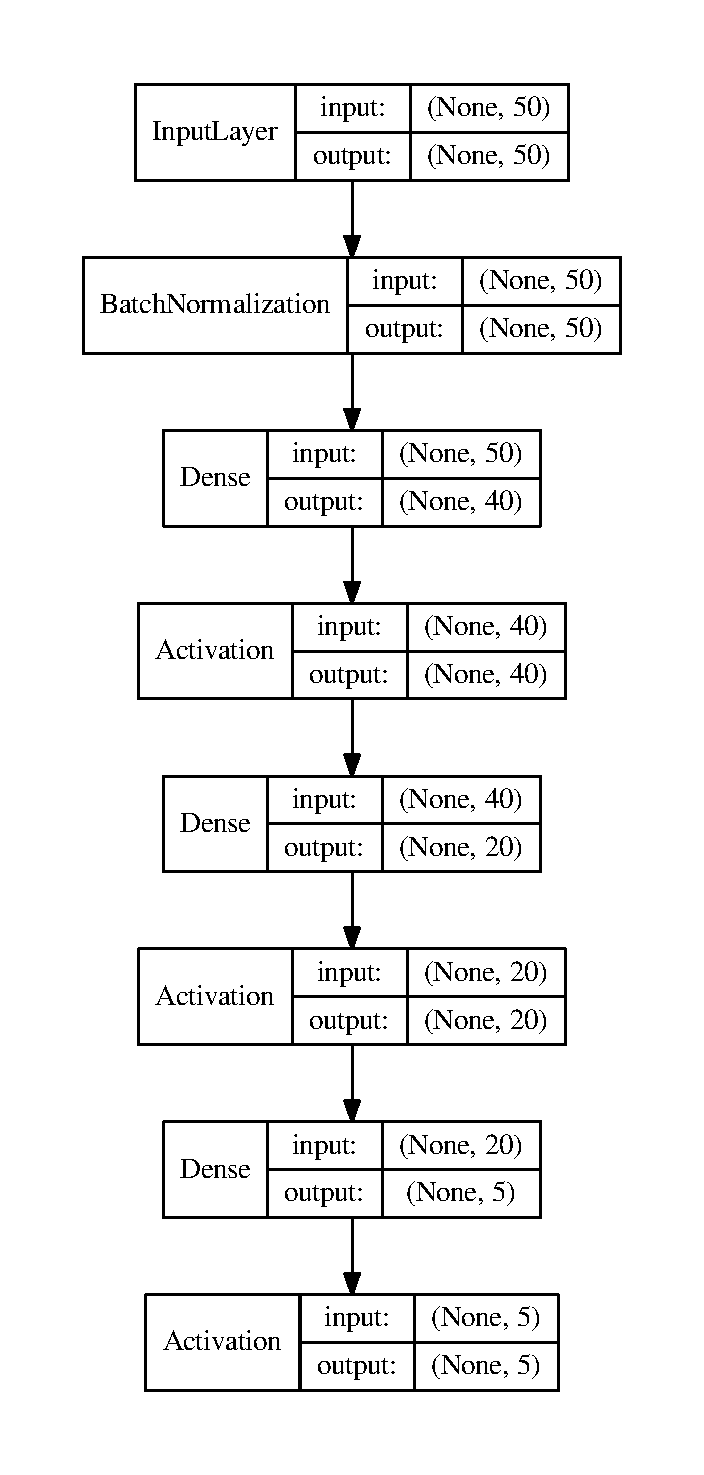
\includegraphics[width=0.99\textwidth]{i1_pam50/model}
\end{minipage}

\end{frame}


\begin{frame}[t]{TCGA-trained PAM50 classifier}{}
	\begin{center}
		\includegraphics<01>[width=0.9\textwidth]{i1_pam50/tsne_train}
		\includegraphics<02>[width=0.9\textwidth]{i1_pam50/tsne_valid}
		\includegraphics<03>[width=0.99\textwidth]{i1_pam50/conf_class_pnorm}
	\end{center}
	
	\Bottom{
		{\only<1>{%
			Unsupervised t-SNE embedding for the training set.
		}}%
		{\only<2>{%
			Unsupervised t-SNE embedding for the test set.
		}}%
		{\only<3>{%
			Confusion matrices for the training set and the test set.
		}}%
	}
\end{frame}


\begin{frame}[t]{TCGA-trained PAM50 classifier}{}
	\begin{center}
		\includegraphics<01>[width=0.9\textwidth]{i1_pam50/expression-heatmap/Normal}
		\includegraphics<02>[width=0.9\textwidth]{i1_pam50/expression-heatmap/LumA}
		\includegraphics<03>[width=0.9\textwidth]{i1_pam50/expression-heatmap/LumB}
		\includegraphics<04>[width=0.9\textwidth]{i1_pam50/expression-heatmap/Her2}
		\includegraphics<05>[width=0.9\textwidth]{i1_pam50/expression-heatmap/Basal}
	\end{center}
	
	\Bottom{
% 		Gene expression heatmaps.
		Normalization sample-wise, then global z-score gene-wise.
	}
\end{frame}

%%%

\begin{frame}[t]{Application of the classifier to BCXX}{}
	\footnotesize
	From 
	``Nanogrid single-nucleus RNA sequencing reveals phenotypic diversity in breast cancer'', 
	Nature Comm, 2017:
	% https://www.nature.com/articles/s41467-017-00244-w
	\begin{quote}
		We also applied the PAM50 gene signature to \textbf{classify single cells}
		into the five major clinical breast cancer expression subtypes 
		(normal-like, luminal A, luminal B, human epidermal growth factor receptor 2 (Her2) or basal-like). 
% 		The relative frequency shifted slightly in each group, however, it was not significant by concordance test (p value >0.4). 
		[..]
		These data showed that most of the single cells and nuclei were classified as Her2 positive, 
		consistent with the report that SK-BR-3 is a Her2-positive cell line by immunohistochemistry. 
		However, we also found that a subset of the single cells were classified as 
		luminal B (10.7, 23.6\%), basal-like (1.8, 5.9\%), normal-like (0.4, 1.4\%), or luminal A (2.4, 3.3\%) 
% 		in both the nuclei and cells (frequency concordance P > 0.4), 
		[..]
		suggesting that the population of cells represented a composite mixture of molecular subtypes.
	\end{quote}
\end{frame}

\begin{frame}[t]{Application of the classifier to BCXX}{}
	\begin{center}
		\includegraphics<01>[width=0.99\textwidth]{i2_pam50_bcxx/pred_singlecell/samples}
	\end{center}
	
	\begin{itemize}
	\item
		BC01--BC03: ER+
	\item
		BC03--BC06: HER2+
	\item
		BC07--BC11: TNBC
	\end{itemize}
\end{frame}

%%%

\begin{frame}[t]{Application of the classifier to BCXX}{}
	\begin{center}
		\includegraphics<01>[width=0.9\textwidth]{i2_pam50_bcxx/pred_singlecell/bygroup/BC01}
		\includegraphics<02>[width=0.9\textwidth]{i2_pam50_bcxx/pred_singlecell/bygroup/BC02}
		\includegraphics<03>[width=0.9\textwidth]{i2_pam50_bcxx/pred_singlecell/bygroup/BC03}
		\includegraphics<04>[width=0.9\textwidth]{i2_pam50_bcxx/pred_singlecell/bygroup/BC03LN}
		\includegraphics<05>[width=0.9\textwidth]{i2_pam50_bcxx/pred_singlecell/bygroup/BC04}
		\includegraphics<06>[width=0.9\textwidth]{i2_pam50_bcxx/pred_singlecell/bygroup/BC05}
		\includegraphics<07>[width=0.9\textwidth]{i2_pam50_bcxx/pred_singlecell/bygroup/BC06}
		\includegraphics<08>[width=0.9\textwidth]{i2_pam50_bcxx/pred_singlecell/bygroup/BC07}
		\includegraphics<09>[width=0.9\textwidth]{i2_pam50_bcxx/pred_singlecell/bygroup/BC07LN}
		\includegraphics<10>[width=0.9\textwidth]{i2_pam50_bcxx/pred_singlecell/bygroup/BC08}
		\includegraphics<11>[width=0.9\textwidth]{i2_pam50_bcxx/pred_singlecell/bygroup/BC09}
		\includegraphics<12>[width=0.9\textwidth]{i2_pam50_bcxx/pred_singlecell/bygroup/BC09_Re}
		\includegraphics<13>[width=0.9\textwidth]{i2_pam50_bcxx/pred_singlecell/bygroup/BC10}
		\includegraphics<14>[width=0.9\textwidth]{i2_pam50_bcxx/pred_singlecell/bygroup/BC11}
		\\
		\includegraphics<01>[width=0.9\textwidth]{i2_pam50_bcxx/pred_bulk/bygroup/BC01}
		\includegraphics<02>[width=0.9\textwidth]{i2_pam50_bcxx/pred_bulk/bygroup/BC02}
		\includegraphics<03>[width=0.9\textwidth]{i2_pam50_bcxx/pred_bulk/bygroup/BC03}
		\includegraphics<04>[width=0.9\textwidth]{i2_pam50_bcxx/pred_bulk/bygroup/BC03LN}
		\includegraphics<05>[width=0.9\textwidth]{i2_pam50_bcxx/pred_bulk/bygroup/BC04}
		\includegraphics<06>[width=0.9\textwidth]{i2_pam50_bcxx/pred_bulk/bygroup/BC05}
		\includegraphics<07>[width=0.9\textwidth]{i2_pam50_bcxx/pred_bulk/bygroup/BC06}
		\includegraphics<08>[width=0.9\textwidth]{i2_pam50_bcxx/pred_bulk/bygroup/BC07}
		\includegraphics<09>[width=0.9\textwidth]{i2_pam50_bcxx/pred_bulk/bygroup/BC07LN}
		\includegraphics<10>[width=0.9\textwidth]{i2_pam50_bcxx/pred_bulk/bygroup/BC08}
		\includegraphics<11>[width=0.9\textwidth]{i2_pam50_bcxx/pred_bulk/bygroup/BC09}
		\includegraphics<12>[width=0.9\textwidth]{i2_pam50_bcxx/pred_bulk/bygroup/BC09_Re}
		\includegraphics<13>[width=0.9\textwidth]{i2_pam50_bcxx/pred_bulk/bygroup/BC10}
		\includegraphics<14>[width=0.9\textwidth]{i2_pam50_bcxx/pred_bulk/bygroup/BC11}
	\end{center}
\end{frame}

%%%


\begin{frame}[t]{Application of the classifier to BCXX}{Artificially assembled tumors}
	{\only<1>{%
		Assemble an artificial ``tumor'':
		\begin{itemize}
		\item
			choose a subtype \[ \text{T $=$ Normal, LumA, LumB, Her2, Basal;} \]
		\item
			collect BCXX cells classified as T with confidence $\leq c_0$;
		\item
			keep only the top 20 cells;
		\item
			bulk expression $:=$ $\sum_{\text{20 cells}}$ [single cell expression $\times$ spike-in].
		\end{itemize}
		
		{\ }
		
		Is this ``tumor'' still classified as T?
	}}%
	{\only<2->{%
		\begin{center}
			\includegraphics<2>[width=0.8\textwidth]{i2_pam50_bcxx/pred_sc2bulk/img/conf-win=5}
			\includegraphics<3>[width=0.8\textwidth]{i2_pam50_bcxx/pred_sc2bulk/img/conf-win=4}
			\includegraphics<4>[width=0.8\textwidth]{i2_pam50_bcxx/pred_sc2bulk/img/conf-win=3}
			\includegraphics<5>[width=0.8\textwidth]{i2_pam50_bcxx/pred_sc2bulk/img/conf-win=2}
			\includegraphics<6>[width=0.8\textwidth]{i2_pam50_bcxx/pred_sc2bulk/img/conf-win=1}
			\includegraphics<7>[width=0.8\textwidth]{i2_pam50_bcxx/pred_sc2bulk/img/conf-win=0}
		\end{center}
		
		{\only<5->{%
			A collection of 20 weakly-LumB cells is frequently classified as LumB.
		}}%
	}}%
\end{frame}

%%%


\begin{frame}[t]{PAM50 LumB subtype: bulk vs sc}{}
	Is LumB 
	\begin{itemize}
	\item<1->
		a ``legitimate'' subtype detectable from (the mRNA of) a single cell? 
		
		Then:
		
		\begin{itemize}
		\item
			False-(+)
			for
			bulk measurement of mixture of other subtypes:
			
			\begin{table}[]
			\centering
			\begin{tabular}{c|cc|c|c}
				& cell 1 & cell 2 & bulk & LumB \\ \hline
			gene X & 1     & 0     & 1    & 1    \\
			gene Y & 0     & 1     & 1    & 1   
			\end{tabular}
			\end{table}
		\item
			Need sc-seq to avoid false-(+).
		\end{itemize}
		
	\item<2->
		a ``bogus'' subtype that arises only as a mixture of other subtypes? 
		
		Then:
		
		\begin{itemize}
		\item
			A single cell is not predictive of LumB subtype.
		\item
			LumB may be more effectively treated as multiple cancers.
		\item
			Need sc-seq to establish the composition of the tumor.
		\end{itemize}
	\end{itemize}
	
\end{frame}


%%%%%%%%%%%%%%%%%%%%%%%%%%%%%%%%%%%%%%%%%%%%%%%%%%%%%%%%%%%%%%%%%%%%%%%%%%%%%%%%%
%\section{Extra}
%%%%%%%%%%%%%%%%%%%%%%%%%%%%%%%%%%%%%%%%%%%%%%%%%%%%%%%%%%%%%%%%%%%%%%%%%%%%%%%%%
%
%
\newcounter{finalframe}
\setcounter{finalframe}{\value{framenumber}}
% Backup frames follow
%
%
%\begin{frame}
%	Appendix
%\end{frame}
%
%%
%
%\begin{frame}
%	%
%\end{frame}
%
%
% FINAL SLIDE
\setbeamercolor{background canvas}{bg=black}
\begin{frame}[plain,b]
	\hfill
	\tiny
	\color{gray}
	this slide is intentionally left blank
\end{frame}
\setbeamercolor{background canvas}{bg=white}


%%%%%%%%%%%%%%%%%%%%%%%%%%%%%%%%%%%%%%%%%%%%%%%%%%%%%%%%%%%%%%%%%%%%%%%%%%%%%%%%%
%\section{Bibliography}
%%%%%%%%%%%%%%%%%%%%%%%%%%%%%%%%%%%%%%%%%%%%%%%%%%%%%%%%%%%%%%%%%%%%%%%%%%%%%%%%%

% {
% \tiny
% \bibliography{../../../r/refs}
% }


%%%%%%%%%%%%%%%%%%%%%%%%%%%%%%%%%%%%%%%%%%%%%%%%%%%%%%%%%%%%%%%%%%%%%%%%%%%%%%%%
\setcounter{framenumber}{\value{finalframe}}
\end{document}
%%%%%%%%%%%%%%%%%%%%%%%%%%%%%%%%%%%%%%%%%%%%%%%%%%%%%%%%%%%%%%%%%%%%%%%%%%%%%%%%
%%%%%%%%%%%%%%%%%%%%%%%%%%%%%%%%%%%%%%%%%%%%%%%%%%%%%%%%%%%%%%%%%%%%%%%%%%%%%%%%

